\documentclass[a4paper,12pt,oneside]{report}

\usepackage[T1]{fontenc} \usepackage{lmodern} \usepackage[utf8]{inputenc}
\usepackage[english]{babel} \usepackage{csquotes}
\usepackage{float} \usepackage{graphicx,subcaption}
\usepackage{amssymb,amsmath} \usepackage{siunitx}
\usepackage[style=numeric,backend=biber]{biblatex} \bibliography{refs}
\usepackage[top=4cm,bottom=4cm,right=4cm,left=4cm,headheight=15pt]{geometry}
%\usepackage[top=4cm,bottom=4cm,outer=3cm,inner=4cm]{geometry}
\usepackage{fancyhdr} \pagestyle{fancy} %\usepackage{lastpage}
%\usepackage{parskip} \setlength{\parindent}{0em} \setlength{\parskip}{1em}
\usepackage{fixltx2e}  % For \lagtextsubscript{}.
\usepackage[colorlinks=true,allcolors=black]{hyperref} \hypersetup{
	pdfauthor={Michaël Defferrard},
	pdftitle={Structured Auto-Encoder},
	pdfsubject={Master Thesis in Information Technologies}
}

\fancyhead[L]{\nouppercase{\leftmark}}
\fancyhead[R]{}
\fancyfoot[C]{\thepage}
%\lhead{Audio Classification with Structured Deep Learning} \chead{} \rhead{}
%\cfoot{-- \thepage --}

\usepackage[acronym]{glossaries} \makeglossaries
\newacronym{EPFL}{EPFL}{École Polytechnique Fédérale de Lausanne}
\newacronym{ICASSP}{ICASSP}{International Conference on Acoustics, Speech and Signal Processing}
\newacronym{CS}{CS}{Compressed Sensing}
\newacronym{ANNs}{ANNs}{Artificial Neural Networks}
\newacronym{CNN}{CNN}{Convolutional Neural Network}
\newacronym{RNN}{RNN}{Recursive Neural Network}
\newacronym{LSTM}{LSTM}{Long Short Term Memory}
\newacronym{MLP}{MLP}{Multi-Layer Perceptron}
\newacronym{RBM}{RBM}{Restricted Boltzmann Machine}
\newacronym{DBN}{DBN}{Deep Belief Network}
\newacronym{MIR}{MIR}{Music Information Retrieval}
\newacronym{MGR}{MGR}{Music Genre Recognition}
\newacronym{MIREX}{MIREX}{Music Information Retrieval Evaluation eXchange}
\newacronym{PSD}{PSD}{Predictive Sparse Decomposition}
\newacronym{CQT}{CQT}{Constant-Q Transform}
\newacronym{LCN}{LCN}{Local Contrast Normalization}
\newacronym{SVM}{SVM}{Support Vector Machine}
\newacronym{RIP}{RIP}{Restricted Isometry Property}
\newacronym{MP}{MP}{Matching Pursuit}
\newacronym{BP}{BP}{Basis Pursuit}
\newacronym{FISTA}{FISTA}{Fast Iterative Shrinkage-Thresholding Algorithm}
\newacronym{ADMM}{ADMM}{Alternating Direction Method of Multipliers}
\newacronym{PD}{PD}{Primal-Dual}
\newacronym{SGD}{SGD}{Stochastic Gradient Descent}
\newacronym{GPU}{GPU}{Graphical Processing Unit}
\newacronym{LASSO}{LASSO}{Least Absolute Shrinkage and Selection Operator}
\newacronym{AGC}{AGC}{Automatic Gain Control}
\newacronym{kNN}{kNN}{k Nearest Neighbors}
\newacronym{PCA}{PCA}{Principal Component Analysis}
\newacronym{NLDR}{NLDR}{Non-Linear Dimensionality Reduction}
\newacronym{SOM}{SOM}{Self-Organizing Map}
\newacronym{LLE}{LLE}{Locally-Linear Embedding}
\newacronym{OLS}{OLS}{Ordinary Least Squares}

\newcommand{\partref}[1]{Part~\ref{part:#1}}
\newcommand{\chapref}[1]{Chapter~\ref{chap:#1}}
\newcommand{\secref}[1]{Section~\ref{sec:#1}}
\newcommand{\eqnref}[1]{(\ref{eqn:#1})}  % Eqn~(\ref{#1})
\newcommand{\figref}[1]{Figure~\ref{fig:#1}}
\newcommand{\tabref}[1]{Table~\ref{tab:#1}}
\newcommand{\HRule}{\rule{\linewidth}{0.5mm}}

\newcommand{\R}{\mathbb{R}}
\DeclareMathOperator*{\argminop}{arg\,min}
\DeclareMathOperator*{\minimizeop}{minimize}
\DeclareMathOperator*{\proxop}{prox}
\DeclareMathOperator*{\sign}{sign}
\DeclareMathOperator*{\tr}{tr}
\DeclareMathOperator*{\spanning}{span}
\newcommand{\argmin}[1]{\argminop\limits_{#1}}
\newcommand{\minimize}[1]{\minimizeop\limits_{#1} \ }  % or \min
\newcommand{\prox}[1]{\text{prox}_{#1}}
\newcommand{\normT}[1]{\| #1 \|_2^2}
\newcommand{\normO}[1]{\| #1 \|_1}
\newcommand{\normZ}[1]{\| #1 \|_0}
\newcommand{\normF}[1]{\| #1 \|_\text{F}^2}
\newcommand{\inner}[2]{\langle #1 , #2 \rangle}
\renewcommand{\L}{\mathbf{L}}
\newcommand{\I}{\mathbf{I}}
\newcommand{\A}{\mathbf{A}}
\newcommand{\D}{\mathbf{D}}
\newcommand{\E}{\mathbf{E}}
\newcommand{\X}{\mathbf{X}}
\newcommand{\Z}{\mathbf{Z}}
\renewcommand{\d}{\mathbf{d}}
\newcommand{\e}{\mathbf{e}}
\newcommand{\x}{\mathbf{x}}
\newcommand{\y}{\mathbf{y}}
\newcommand{\z}{\mathbf{z}}
\newcommand{\eps}{\mathbf{\epsilon}}
\newcommand{\gam}{\mathbf{\Gamma}}
\newcommand{\Eone}{E_1(\Z, \D)}
\newcommand{\Etwo}{E_2(\Z, \D)}
\newcommand{\Ethree}{E_3(\Z, \D, \E)}
\newcommand{\Xx}{\mathcal{X}}
\newcommand{\G}{\mathcal{G}}
\newcommand{\V}{\mathcal{V}}
\newcommand{\W}{\mathbf{W}}
\newcommand{\set}[2]{\{#1_i\}_{i=1}^#2}
\newcommand{\st}{\text{ s.t. }}
\newcommand{\cst}[2]{\|#1_#2\|_2 \leq 1}
%\newcommand{\forallx}[2]{\forall #1 \in \{1,\ldots,#2\}}
\newcommand{\forallx}[2]{#1 = 1, \ldots, #2}
%\newcommand{\forallx}[2]{\|#1_#2\|_2 \leq 1 \text{ for } #2 = 1,\ldots,#3}
\newcommand{\cstd}{\cst{\d}{i}, \ \forallx{i}{m}}
\newcommand{\cste}{\cst{\e}{k}, \ \forallx{k}{n}}
\newcommand{\pd}[2]{\frac{\partial #1}{\partial #2}}
\newcommand{\fd}{f_d(\Z, \D)}
\newcommand{\fz}{f_z(\Z)}
\newcommand{\fg}{f_g(\Z)}
\newcommand{\fe}{f_e(\Z, \E)}



%%%%%%%%%%%%%%%%%%%%%%%%%%%%%%%%%%%%%%%%%%%%%%%%%%%%%%%%%%%%%%%%%%%%%%%%%%%%%%%


\begin{document}

%\hypersetup{pageanchor=false}
\begin{titlepage}
	
	
\includegraphics[height=2.5cm]{img/logo_epfl}
	\hfill
	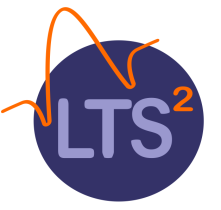
\includegraphics[height=2.5cm]{img/logo_lts2}
	\vspace{1.2cm}
	
	\begin{center}
		
		\textsc{\LARGE MASTER THESIS}\\
		\vspace{0.5cm}
		\large Electrical and Electronic Section\\
		\large Major in Information Technologies\\
		\vspace{0.8cm}
		
		\HRule
		\vspace{0.9cm}
		\textsc{\Huge Structured Auto-Encoder}\\
		\vspace{0.5cm}
		\textsc{\Large with application to}\\
		\vspace{0.2cm}
		\textsc{\Large Music Genre Recognition}\\
		\vspace{0.6cm}
		\HRule
		\vspace{1.3cm}
		
		\begin{minipage}{0.45\textwidth}
			\begin{flushleft} \large
				\textbf{Student}\\ \vspace{0.5ex}
				Michaël \textsc{Defferrard} \\ \vspace{2.5ex}
				\textbf{Professor} \\ \vspace{0.5ex}
				Pierre \textsc{Vandergheynst}
			\end{flushleft}
		\end{minipage}
		\begin{minipage}{0.45\textwidth}
			\begin{flushright} \large
				\textbf{Supervisors} \\ \vspace{0.5ex}
				Xavier \textsc{Bresson} \\ \vspace{0.2ex}
				Johan \textsc{Paratte}
			\end{flushright}
		\end{minipage}
		
		\vspace{1.5cm}
		\large EPFL LTS2 Laboratory\\
		\vspace{0.8cm}
		\large June 19, 2015
		
	\end{center}
	
\end{titlepage}
%\hypersetup{pageanchor=true}


%%%%%%%%%%%%%%%%%%%%%%%%%%%%%%%%%%%%%%%%%%%%%%%%%%%%%%%%%%%%%%%%%%%%%%%%%%%%%%%

% No new page for the abstract in report class.
\def\abstract{
	\vfil
	\begin{center}
		{\bfseries \abstractname\vspace{-.5em}}
	\end{center}
	\quotation
}
\def\endabstract{\par
	\endquotation
}

\pagestyle{empty}
\begin{abstract}
	In this work, we introduce a novel auto-encoder architecture which leverages on the recent advances of deep learning using an efficient auto-encoder strategy that simultaneously learns sparse representation of inputs and dictionary adapted to those inputs. Our main goal is to find a solution to sparse coding that is structured by the proximities of the sparse features encoded by a graph of audio inputs. We borrow ideas from manifold learning to constrain our solution to be smooth on this graph, i.e. to have a small Dirichlet energy, in order to implicitly force feature proximities. Our auto-encoder model is formulated as a non-convex optimization problem, for which a well-posed iterative scheme is provided.
\end{abstract}

\renewcommand{\abstractname}{Acknowledgements}
\begin{abstract}
	I would first like to thank Dr. Xavier Bresson for his dedicated day-to-day supervision, which included a weekly meeting during which we discussed the achieved results and debated new ideas. He further provided me with many inputs, intuitions and references, which were very helpful to clarify some concepts. Finally, I want to thank him for his review of parts of this manuscript.

	I would also like to thank Johan Paratte for his helpful intuitions at the beginning of the project and his advices on how to structure the thesis.

	Finally, I would like to thank Prof. Pierre Vandergheynst which has made this very interesting project possible. Thanks to him and this project, I've learned much more that the content of this thesis.
\end{abstract}

\tableofcontents
\pagestyle{fancy}

%\printglossaries
%\addcontentsline{toc}{chapter}{Glossary}
%\addcontentsline{toc}{chapter}{Acronyms}


%%%%%%%%%%%%%%%%%%%%%%%%%%%%%%%%%%%%%%%%%%%%%%%%%%%%%%%%%%%%%%%%%%%%%%%%%%%%%%%


\chapter*{Introduction}
\addcontentsline{toc}{chapter}{Introduction}

{\color{red} Introduction to the matter.}
%\chapter{Machine learning}
% What's the purpose of learning.
% Why learned features instead of hand-crafted features ?
%\section{Supervised vs unsupervised}
% Explain the difference. Why do we want unsupervised ?


% What will be presented. Design goal.
This thesis introduces the \textit{structured auto-encoder}, an auto-encoder variant which preserves the structure of the data while transforming it in a sparse representation. It learns sparse representations that explicitly take into account the local manifold structure of the data.
The primary goal of the proposed algorithm is unsupervised representation learning toward the goal of feature extraction, while being robust to noisy data and fast at feature extraction (after the training phase). As the discriminative power of learned representations cannot be directly evaluated, the proposed algorithm shall be evaluated through a classification task.
We propose an application in \gls{MIR} which consists of retrieving the genre of unknown musical clips. The proposed algorithm 

%As we shall see, it has the properties of an hybrid between a sparse auto-encoder \cite{lecun2006sparseAutoencoders, ranzato2007stackedSparseAutoencoders} and a denoising auto-encoder \cite{bengio2008denoisingAutoencoders}.

% Plan.
This thesis is divided in two parts. Through \partref{algorithm},
%the proposed model is introduced by a motivation in \chapref{motivation}
some background informations are given in \chapref{background} and the proposed model is
constructed step by step in \chapref{model}, which is the core of this work. A well-posed iterative scheme to solve the resulting non-convex optimization problem is then proposed in \chapref{optimization}. That is the way the model is learned. % while \chapref{related_work} compares it to existing models.
\secref{approximate_schemes} shows how features may be extracted with the learned data model.
As a testbed of our algorithm's performance, an application to \gls{MGR} is proposed in \partref{application} with a presentation of the problem in \chapref{problem}, our proposed system in \chapref{system}
% along with some implementation details in \chapref{implementation}.
\chapref{results} is dedicated to the presentation of the experimental results.



This work was accomplished as a Master thesis, which is an integral part of the major in Information Technologies curriculum from the Electrical and Electronic Section of the \gls{EPFL}. It was conducted at the LTS2 laboratory\footnote{The laboratory homepage is accessible at \url{http://lts2www.epfl.ch/}.}.

While the project was ongoing, I continuously published my thoughts, observations, findings, experiments, results and plans as well as a summary of the weekly meetings with my supervisors on an online blog\footnote{My research blog is available at \url{https://lts2research.epfl.ch/blog/mdeff/}.} in the format of an open laboratory notebook. In the spirit of open research, the code as well as all the results, this report and the ongoing paper are versioned with git and available online through GitHub\footnote{My GitHub account can be found at \url{https://github.com/mdeff}.}. Some continuation of this work shall be submitted to the 41st IEEE \gls{ICASSP}. We may also aim at a journal paper at the end of the project.

This manuscript is available on GitHub, git revision ***


%%%%%%%%%%%%%%%%%%%%%%%%%%%%%%%%%%%%%%%%%%%%%%%%%%%%%%%%%%%%%%%%%%%%%%%%%%%%%%%


\part{Algorithm} \label{part:algorithm}
% Define the structuring auto-encoder.

\chapter{Motivation} \label{chap:motivation}
% Why ? Neural nets, deep learning, unsupervised feature extraction, representation learning.

\section{Neural networks}
% Why ? Distributed representation and computation (e.g. training on GPU, clusters) --> much what symbolic AI is not (mainly search algorithms, SAT solvers)
% Started in the late 1950s with the perceptron.

\gls{ANNs} are a family of statistical learning models inspired by biological neural networks and are used to estimate or approximate functions that can depend on a large number of inputs and are generally unknown. It is presented as a network of interconnected neurons whose connections have numeric weights that can be tuned based on experience. It makes the neural nets adaptive to inputs and capable of learning.

% What is it ? In general.
Such a network is composed by an input layer, a number of hidden layers and an output layer. The activation of the neurons in the input layer corresponds to the input vector, e.g. an image for computer vision, a song for \gls{MIR}, a word vector for machine translation and sentiment analysis. A weight matrix, followed by a non-linear activation function, then transforms the vector in another representation. The output vector of the first layer is the input vector of the second, and so on until the output layer is reached. The activation of the neurons in the output layer may represent classes, probability distributions, or the estimated value of an unknown function to be learned.

{\color{red} Picture ?}

% Types: feed-forward or recurrent
In a feed-forward network, the connections go from one layer to the next, i.e. information only goes in one direction, forward, from the input nodes, through the hidden nodes (if any) and to the output nodes. Such networks are known to be able to approximate any function. The perceptron, the \gls{MLP} and the \gls{CNN} are examples of this class of networks.
By introducing backward connections, i.e. the connections between units form a directed cycle, we obtain a so called \gls{RNN}. This creates an internal state of the network which allows it to exhibit dynamic temporal behavior. Unlike feed-forward neural networks, an \gls{RNN} can use its internal memory to process arbitrary sequences of inputs. It is known to be able to approximate any program. Such networks have proven very successful for machine translation.

% How to train, supervised.
In a supervised learning setting, the network is trained by back-propagating the error, gradient based learning method, from the output layer to the input through all the hidden layers.
The vanishing gradient problem, where errors shrink exponentially with the number of layers as they propagate from layer to layer, is a major issue of the algorithm \cite{hochreiter2001vanishingGradient}. Various methods, like unsupervised pre-training or \gls{LSTM} \cite{hochreiter1997LSTM}, were developed to work around this problem.

% How to train, unsupervised.
However, in an unsupervised learning setting, there is no desired output, which implies that there is no error to back-propagate. The training algorithm should thus optimize for another objective, which represent desired properties about the output. We will introduce next such an algorithm, called an auto-encoder.

\section{Auto-encoders} \label{sec:auto_encoders}
% For unsupervised learning, i.e. feature extraction.
% Auto-encoders as a manifold learning tool (Bengio review).

An auto-encoder, auto-associator or Diabolo network is an artificial neural network composed of $n$ input and output units and $m$ hidden units. It is used for learning efficient codings \cite{bourlard1988autoencoder, hinton1994autoencoder}. The aim of an auto-encoder is to learn a distributed representation (encoding) for a set of data. An auto-encoder is trained to encode the input $\x \in \R^n$ into some representation $\z \in \R^m$ so that the input can be reconstructed from that representation. It is thus a generative model. Hence the target output of the auto-encoder is the auto-encoder input itself. Auto-encoders may further be stacked to form a \gls{DBN}, while each layer can be trained separately \cite{bengio2007DBN, ranzato2007stackedSparseAutoencoders}.
% Stacked Auto-Encoders, not DBN

{\color{red} Picture ?}

% if linear activations are used, or only a single sigmoid hidden layer, then the optimal solution to an auto-encoder is strongly related to principal component analysis (PCA).[5]
If there is one linear hidden layer and the mean squared error criterion is used to train the network, then the $k$ hidden units learn to project the input in the span of the first $k$ principal components of the data \cite{bourlard1988autoencoder}. If the hidden layer is non-linear, the auto-encoder behaves differently from PCA, with the ability to capture multi-modal aspects of the input distribution \cite{japkowicz2000autoencoderPCA}.

The hope is that the code $\z$ is a distributed representation that captures the main factors of variation in the data: because $\z$ is viewed as a lossy representation of $\x$, it cannot be a good representation (with small loss) for all $\x$. So learning drives it to be one that is a good representation in particular for training examples, and hopefully for others as well (and that is the sense in which an auto-encoder generalizes), but not for arbitrary inputs.

It can typically be used for dimensionality reduction by learning a compressed ($m<n$) representation of the data. Another application is feature extraction before classification, for which we want an higher dimensionality ($m>n$) for easier separability. One serious issue with this approach is that if there is no other constraint, then an auto-encoder with $n$-dimensional input and an encoding of dimension $m \geq n$ could potentially just learn the identity function. There are different ways that an auto-encoder with more hidden units than inputs could be prevented from learning the identity, and still capture something useful about the input in its hidden representation $\z$.

\paragraph{Sparse auto-encoders.}
Another strategy, based on the concept of sparse coding, is to add a sparsity constraint on the code. While an ordinary auto-encoder or an \gls{RBM} has an encoder part which computes $P(\z|\x)$ and a decoder part which computes $P(\x|\z)$, sparse coding systems only parametrize the decoder: the encoder is implicitly defined as the solution of an optimization. A middle ground between ordinary auto-encoders and sparse coding was proposed in \cite{lecun2006sparseAutoencoders, ranzato2007stackedSparseAutoencoders} and applied to pattern recognition and machine vision tasks. They propose to let the codes $\z$ be free (as in sparse coding algorithms), but include a parametric encoder (as in an ordinary auto-encoder or \gls{RBM}) and a penalty for the difference between the free non-parametric codes $\z$ and the outputs of the parametric encoder. In this way, the optimized codes $\z$ try to satisfy two objectives: reconstruct well the input (like in sparse coding), while not being too far from the output of the encoder (which is stable by construction, because of the simple parametrization of the encoder). See \secref{encoder} for the definition of our encoder.

\paragraph{Denoising auto-encoders.}
One strategy is to add noise in the encoding. The denoising auto-encoder thus minimizes the error in reconstructing the input from a stochastically corrupted transformation of the input \cite{bengio2008denoisingAutoencoders}. Intuitively, a denoising auto-encoder does two things: try to encode the input (preserve the information about the input), and try to undo the effect of a corruption process stochastically applied to the input of the auto-encoder. This is essentially what a \gls{RBM} does \cite{hinton2002RBM}.


%%%%%%%%%%%%%%%%%%%%%%%%%%%%%%%%%%%%%%%%%%%%%%%%%%%%%%%%%%%%%%%%%%%%%%%%%%%%%%%


\chapter{Model} \label{chap:model}
% Step by step construction: sparse coding, dictionary learning, encoder learning, manifold learning.
% Xavier: maybe not useful as it is just the enumeration of the sub-titles of chapter 2 --> give instead a global motivation.

This chapter presents the proposed structured auto-encoder. \secref{assumptions} states the assumptions of the model. \secref{linear_regression} reviews the basics of linear regression, the foundation of our model. \secref{sparse_coding} introduces sparse coding, \secref{dictionary_learning} introduces a trainable dictionary and \secref{manifold_learning} introduces manifold learning. Last but not least, \secref{encoder} introduces the trainable encoder. Finally, \secref{energy_formulation} reviews the whole energy-based formulation and brings some new insights.

\section{Assumptions} \label{sec:assumptions}
% Xavier: needs to be improved.

\paragraph{Sparse representation.}
We make the hypothesis that a set of sample signals drawn from the same distribution can be sparsely represented in some frame\footnote{A frame of a vector space is a set of vectors which may be linearly dependent. It is a generalization of a basis.}. Each signal should be approximately reconstructed by a linear combinations of a few atoms from a suitable dictionary. As we shall see, this dictionary may be adaptive and learned directly from the data. Sparsity has become a concept of great interest recently, not only in machine learning but also in statistics and signal processing, in particular with the work on \gls{CS} \cite{candes2005CS, donoho2006CS}.
% There is a huge body of literature on sparse coding and compressed sensing to support this hypothesis.
% --> sparse coding.

% Structured: adding similarity information between inputs.
% Manifold: not all possible signals are reasonable / feasible.
% Xavier: a definition of auto-encoder should be given before in the report.
% We further assume that the subspace spanned by the data is much smaller than the Euclidean space.
\paragraph{Structured data.}
Our second hypothesis is that the dataset holds some structure, in the sense that related samples are close to each other (with respect to some metric). Given a large enough training set, the structure of the data distribution should be able to be captured; i.e. a new valid sample (e.g. from the testing set) should be close to the seen examples. It suggests that the data lie on a lower dimensional manifold embedded in a high dimensional vector space. This manifold is however often unknown and must be learned. \gls{SOM} \cite{kohonen1982SOM}, \gls{LLE} \cite{roweis2000LLE}, Laplacian Eigenmaps \cite{belkin2001laplacianEigenmaps} and Isomap \cite{tenenbaum2000isomap} are some popular techniques which learn manifolds in a \gls{NLDR} framework. Auto-encoders used for dimensionality reduction are able to learn a map from high to low-dimensional space with fewer hidden units than inputs. They are trained to learn to optimally encode the input vectors into a small number of dimensions and decode them back into the original space with minimal error \cite{bourlard1988autoencoder}.
% --> manifold learning.

\paragraph{Encoder.}
We further make the assumption that a simple encoder can be trained to avoid the need of an optimization process that extracts the features during testing, i.e. after the training phase. The encoder shall be more efficient than the optimization process while not degrading too much the quality of the extracted features. Note that even if this hypothesis is not verified, the algorithm is still an auto-encoder, although with an implicit encoder.
% --> auto-encoder.

\section{Linear regression} \label{sec:linear_regression}

\paragraph{Model.}
Given a set $\set{\x}{N} \in \R^n$ of $N$ signals, the subspace $\Xx = \spanning \{\x_i\}_{i=1}^N \subset \R^n$ is defined as the subspace spanned by the data. Then, given a signal $\x \in \Xx$ and a frame $\D \in \R^{n \times m}$, we want to find a representation $\z \in \R^m$ which satisfies the linear regression model
\begin{equation} \label{eqn:linear_regression}
	\x = \D \z + \eps,
\end{equation}
where $\mathbf{\epsilon} \in \R^n$ is the reconstruction error, which is not negligible as long as the frame $\D$ is not complete on $\Xx$.

\paragraph{Capacity.} The hyper-parameter $m$ defines the learning capacity of the auto-encoder. A capacity $m < n$ is good for dimensionality reduction as it exploits the statistical regularities present in the training set while being more compact. A capacity $m > n$ is good for classification as it allows for an easier (linear) separability enabled by the higher dimensional space.

\begin{figure}[ht]
	\centering
	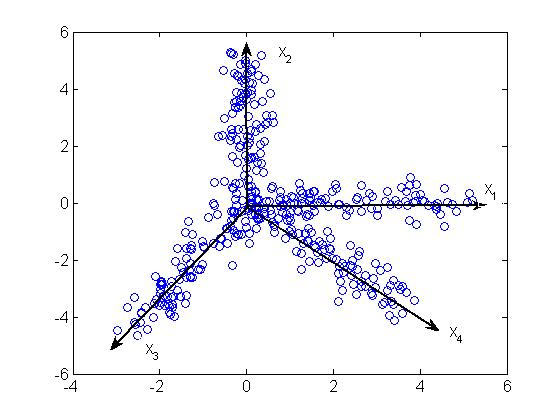
\includegraphics[height=6cm]{img/overcomplete_frame}
	\caption[]{An example of overcomplete frame. While the data lies in a two-dimensional space, a four-dimensional space supported by an overcomplete frame allows a better representation.\footnotemark}
	\label{fig:overcomplete_frame}
\end{figure}
\footnotetext{Figure from Wikipedia.}

\paragraph{Completeness.}
A frame is complete if it can represent any vector $\x \in \Xx$. It is overcomplete if the removal of a vector from the frame results in a complete frame. A set of $n < m$ linearly independent vectors would indeed be overcomplete on the whole space $\R^n$ and a set of $m=n$ linearly independent vectors, like the Fourier transform, would form a basis\footnote{A basis is a set of linearly independent vectors who span the entire space, i.e. it is a linearly independent spanning set.} of $\R^n$, which is obviously complete.

% Complete.
A complete frame which is not overcomplete allows bidirectional lossless transformations. Such problems are well-posed as there exists a unique solution to \eqnref{linear_regression} with $\eps=0$.

% Not complete.
If the frame is not complete, there exist no solution to \eqnref{linear_regression} with $\eps=0$ as the system is overdetermined. An error measure, like \eqnref{least_square} for the \gls{OLS} method, should instead be minimized.

% Overcomplete.
In different research, such as signal processing and function approximation, overcomplete representations have been advocated because they have greater robustness in the presence of noise, can be sparser, and can have greater flexibility in matching structure in the data. However, because of this redundancy, a signal can have multiple expressions under an overcomplete frame \cite{lewicki2000overcompleteRepresentation}. See \figref{overcomplete_frame} for an example of the flexibility of an overcomplete frame to represent a dataset. As there is then an infinite number of solutions to \eqnref{linear_regression} with $\eps=0$, i.e. the problem is ill-posed, a regularization over $\z$ shall be introduced. Optimization techniques are then used to find the optimal solution which minimizes the sum of the error measure and the regularization term, controlled by an hyper-parameter.

\paragraph{Ordinary least squares.}
The method of least squares is a standard approach in regression analysis to the approximate solution of overdetermined systems. "Least squares" means that the overall solution minimizes the sum of the squares of the errors made in the results of every single equation, i.e. it finds
\begin{equation} \label{eqn:least_square}
	\z^* = \argmin{\z} \normT{\x - \D\z},
\end{equation}
where $\normT{\cdot}$ denotes the squared $\ell_2$, or Euclidean, norm. This problem has the closed-form solution
\begin{equation}
	\z^* = (\D^T\D)^{-1} \D^T \x,
\end{equation}
where $T$ denotes the matrix transpose. The primary assumption of \gls{OLS} is that there are zero or negligible errors in the independent variable $\D$, since this method only attempts to minimize the mean squared error in the dependent variable $\x$. That is not an issue in an auto-encoder setting where $\D$ is either hand-crafted or learned.

% underdetermined == ill-posed ?
\paragraph{Regularization.}
% L2.
Tikhonov regularization \cite{tikhonov1963tikhonovRegularization}, or ridge regression, is the most commonly used method of regularization of ill-posed problems. It adds a prior of the form $\lambda \normT{\gam \z}$ to the minimization problem \eqnref{least_square} as follows:
\begin{equation} \label{eqn:tikhonov_regularization}
	\z^* = \argmin{\z} \normT{\x - \D\z} + \lambda \normT{\gam \z},
\end{equation}
where $\gam$ is the Tikhonov matrix. This matrix is often chosen to be a multiple of the identity matrix, i.e. $\gam = \alpha \mathbf{I}$, giving preference to solutions with smaller norms. In a Bayesian context, this is equivalent to placing a zero-mean normally distributed prior on $\z$ \cite{vogel2002inverseProblems}. In other cases, lowpass operators, e.g. a difference operator or a weighted Fourier operator, may be used to enforce smoothness if the underlying vector is believed to be mostly continuous. A regularization of this kind will be introduced in our model in \secref{manifold_learning}. An explicit solution is given by
\begin{equation}
	\z^* = (\D^T\D + \gam^T\gam)^{-1} \D^T \x.
\end{equation}

% L1.
Another commonly used regularization is the \gls{LASSO} \cite{tibshirani1996Lasso}, which adds the prior $\lambda \normO{\z}$ to the minimization problem \eqnref{least_square} as follows:
\begin{equation} \label{eqn:lasso_regularization}
	\z^* = \argmin{\z} \normT{\x - \D\z} + \lambda \normO{\z},
\end{equation}
where $\normO{\z} = \sum_{i=1}^{m} |z_i|$ is the $\ell_1$ norm of $\z$, also called the Taxicab or Manhattan norm.
In a Bayesian context, this is equivalent to placing a zero-mean Laplace prior distribution on $\z$ \cite{park2008BayesianLasso}. The advantage of the \gls{LASSO} is that it promotes the simplest solutions, i.e. the solutions with many zeros. Driving parameters to zero effectively deselects the features from the regression. \gls{LASSO} thus automatically selects the most relevant features, whereas ridge regression never fully discards any. For this reason, the \gls{LASSO} and its variants are fundamental to the field of \gls{CS}. A regularization of this kind will be introduced in our model in \secref{sparse_coding}.

% L1 + L2.
An extension of this approach is the elastic net regularization \cite{zou2005ElasticNet} which linearly combines the $\ell_1$ and $\ell_2$ penalties of the \gls{LASSO} and ridge methods as follows:
\begin{equation} \label{eqn:elasticnet_regularization}
	\z^* = \argmin{\z} \normT{\x - \D\z} + \lambda_2 \normT{\z} + \lambda_1 \normO{\z}.
\end{equation}
This regularization overcomes some limitations of the $\ell_1$ penalty, e.g. the saturation which happens for high-dimensional data with few examples, or the fact that the \gls{LASSO} tends to select only one variable and ignore the others if there is a group of highly correlated variables.

\section{Sparse coding} \label{sec:sparse_coding}
% What it is, why it works, why it's good.
% paper who demonstrates that L1 penalty leads to same solution as L0 while being convex, not combinatorial

% Sparse coding.
The main idea behind sparse coding \cite{olshausen1996SparseV1, mairal2008sparseCoding} is to express the signal $\x \in \Xx \subset \R^n$ as a sparse linear combination of basis functions $\set{\d}{m} \in \R^n$, or atoms, from an overcomplete dictionary $\D \in \R^{n \times m}$. The sparse code $\z^* \in \R^m$ is given by
\begin{equation} \label{eqn:sparsecoding}
	\z^* = \argmin{\z} \frac{\lambda_d}{2} \normT{\x - \D \z} + \lambda_z \normZ{\z},
\end{equation}
where $\normZ{\z}$ denotes the number of non-zero elements in $\z$.  $\lambda_d$ and $\lambda_z$ are the (redundant) hyper-parameters setting the trade-off between the data term, an accurate reconstruction, and the prior, a sparse solution. Overcomplete sparse representations tend to be good features for classification systems as they provide a succinct representation of the signal, are robust to noise and are more likely to be linearly separable due to their high dimensionality.

% Faster sparse coding approximations.
Finding the sparse code $\z^*$ however requires a combinatorial search which is an NP-hard problem, intractable in high dimensional spaces. Various approximations have thus been proposed. Matching Pursuit \cite{mallat1993MatchingPursuit} offers a greedy approximation to the solution while \gls{BP} \cite{chen1998BasisPursuit} is the popular convex approximation
\begin{equation} \label{eqn:basispursuit}
	\z^* = \argmin{\z} \frac{\lambda_d}{2} \normT{\x - \D \z} + \lambda_z \normO{\z},
\end{equation}
which is the \gls{LASSO} regularized least square problem introduced in \eqnref{lasso_regularization}. As is now well understood \cite{candes2005CS, donoho2006CS}, the $\ell_1$ norm is a very good proxy for the $\ell_0$ pseudo-norm and naturally induces sparse results. It can even be shown to recover exactly the true sparse code, i.e. the solution of \eqnref{sparsecoding} (if there is one), under mild conditions \cite{donoho2003OptSparse}. {\color{red}link with \gls{RIP}}. A number of algorithms have been proposed to efficiently solve this problem \cite{chen1998BasisPursuit, beck2009FISTA, ng2006EfficientSparse, li2009Coordinate}. They however still rely on computationally expensive iterative procedures which limit the system's scalability and real-time applications. While a direct method will always be preferred for feature extraction, iterative methods will still be necessary during training. Distributed computing with \gls{GPU} or via cloud computing will hopefully accelerate the process.

\section{Dictionary learning} \label{sec:dictionary_learning}

% Why ?
\paragraph{Model.}
In classical sparse coding, the dictionary is composed of known functions such as sinusoids \cite{bracewell1965fourier}, wavelets \cite{mallat1999wavelet}, Gabors \cite{gabor1946gabor} or gammatones\footnote{A gammatone is a sinusoid (a pure tone) with an amplitude envelope which is a scaled gamma distribution function. It is used to build cochlear models.} \cite{holdsworth1992gammatone}; i.e. hand-crafted features. One may also want to learn a dictionary that is adaptive to the type of data at hand. This approach may allow an even more compact representation and may lead to the discovery of previously unknown discriminative features.

% How ?
To use the dictionary $\D$ as an unknown variable, all the training data shall be part of the objective function as the dictionary depends on all of them. The energy function, composed by an $\ell_2$ fidelity term and an $\ell_1$ penalty, becomes
\begin{equation} \label{eqn:en_dict}
	\Eone = \frac{\lambda_d}{2} \normF{\X - \D \Z} + \lambda_z \normO{\Z},
\end{equation}
where $\normF{\cdot}$ denotes the squared Frobenius norm, $\X = \set{\x}{N} \in \R^{n \times N}$ is the set of training vectors and $\Z = \set{\z}{N} \in \R^{m \times N}$ their associated sparse codes. $N$ is naturally the number of training vectors, which should be much greater than the size $m$ of the dictionary to avoid the trivial solution where examples are copied in the dictionary. The problem to solve is then
\begin{equation} \label{eqn:pr_dict}
	\minimize{\Z,\D} \Eone \st \cstd,
\end{equation}
where the $\ell_2$ ball constraint (usually implemented by rescaling the columns $\d_i$ of $\D$ at each iteration) prevents the trivial solution where the code coefficients go to zero while the bases are scaled up. While this problem is not convex, a good approximate solution can be found by iteratively minimizing for $\Z$ and $\D$ \cite{olshausen1996SparseV1}.
% Simple gradient descent or more sophisticated methods \cite{chen1998BasisPursuit, beck2009FISTA, li2009Coordinate} for $\z$, stochastic gradient descent for $\D$.

\paragraph{Completeness.}
The learned dictionary may be seen as an overcomplete frame of the subspace $\Xx$ spanned by the training data. The overcompleteness of the learned dictionary could indeed be tested: the frame should be able to perfectly represent any training sample, i.e. in the absence of the $\ell_1$ regularization, the reconstruction error $\eps$ of \eqnref{linear_regression} should be zero.

% Motivation: learned dictionaries resemble brain processing stages.
\paragraph{Biological motivation.}
There is evidence that sparse coding may be a strategy employed by the brain in the early stages of visual and auditory processing \cite{olshausen1996SparseV1, olshausen1997SparseV1, smith2006SparseAudio}. Basis functions learned on natural images have been shown to resemble the receptive fields of neurons in the visual cortex \cite{olshausen1996SparseV1, olshausen1997SparseV1}. Basis functions learned on natural sounds were found to be highly similar to gammatone functions \cite{smith2006SparseAudio} which have been used to model the action of the basilar membrane in the inner ear. Moreover, learning on natural time-varying stimuli such as speech or video has been shown to produce localized bases \cite{lewicki2000SparseSpeech, olshausen2000SparseVideo}.

\section{Manifold learning} \label{sec:manifold_learning}

%\subsection{Manifold}

% General introduction.
\paragraph{Manifold.}
In mathematics, a manifold is a topological space that resembles Euclidean space near each point, i.e. each point of an $n$-dimensional manifold has a neighborhood that is homeomorphic to the Euclidean space of dimension $n$. Lines and circles, but not figure eights, are one-dimensional manifolds. Two-dimensional manifolds are also called surfaces. Examples include the plane, the sphere, and the torus, which can all be embedded in three-dimensional real space. \figref{manifolds} shows examples of 1D and 2D manifolds.

\begin{figure}[ht]
	\centering
	\begin{subfigure}[b]{0.49\textwidth}
		\centering
		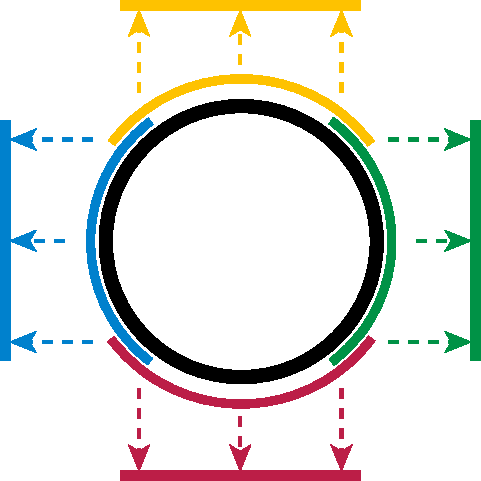
\includegraphics[height=6cm]{img/circle_manifold_charts}
		\caption{}
	\end{subfigure}
	\begin{subfigure}[b]{0.49\textwidth}
		\centering
		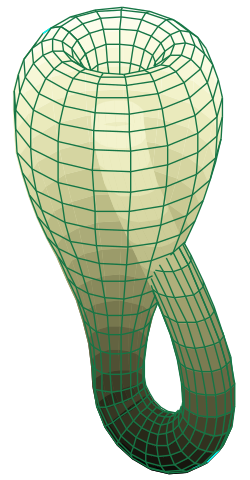
\includegraphics[height=6cm]{img/klein_bottle}
		\caption{}
	\end{subfigure}
	\caption[]{Examples of manifolds.\footnotemark (a) The circle, a 1D manifold, can be mapped by 4 charts. (b) The klein bottle is a 2D manifold that cannot be embedded in a 3D space without self-intersection.}
	\label{fig:manifolds}
\end{figure}
\footnotetext{Figures from Wikipedia.}

% Example close to our case.
Let's imagine a single handwritten digit recognition system. The input is an image of $n \times n$ pixels which is represented by a vector $\x \in \R^{n \times n}$. However, not all vectors $\x \in \R^{n \times n}$ represent meaningful data. The vast majority indeed represents garbage. We may make the hypothesis that the set of plausible digits lies on a $d$-dimensional manifold where $d \leq n \times n$.

% Approximate a manifold.
The problem is that we often ignore the shape of the embedded manifold. We only have at our disposal some samples which are drawn from it, e.g. a few examples of handwritten digits. Another example with object scanning: we obtain a discrete point cloud sampled from the surface. We do know some points on the surface, but we don't know the exact surface.

We use graphs as discrete approximations of low-dimensional manifolds embedded in high-dimensional spaces. The set of data are samples drawn from this unknown manifold.

%\subsection{Spectral graph overview}
%\subsection{Spectral graph theory}
% Paper: Pierre's review

%\section{Graph definition}
% What is a graph --> discrete approximation of a low-dimensional manifold embedded in a high dimensional space.

% General formulation.
\paragraph{Graph.}
Graphs are generic data representation forms which are useful for describing the geometric structures of data domains in numerous applications, including social, energy, transportation, sensor, and neuronal networks. The connectivity and weight associated with each edge in the graph is either dictated by the physics of the problem at hand or inferred from the data; in which case it often represents the similarity between the two vertices it connects. For instance, the edge weight may be inversely proportional to the physical distance between nodes in the network, or proportional to a similarity measure between those nodes. A \textit{graph signal} is a signal which resides on the graph, i.e. a signal with one sample at each vertex of the graph. An example of a graph signal is shown in \figref{example_graph}.

\begin{figure}[ht]
	\centering
	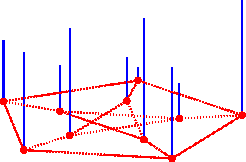
\includegraphics[height=6cm]{img/example_graph}
	\caption[]{A random positive graph signal on the vertices of the Petersen graph. The height of each blue bar represents the signal value at the vertex where the bar originates.\footnotemark}
	\label{fig:example_graph}
\end{figure}
\footnotetext{Figure from \cite{pierre2013graph}.}

Weighted graphs are commonly used to represent similarities between data points in statistical learning problems for applications such as machine vision
[2] and automatic text classification [3].

We first review some basic definitions and notations from spectral graph theory and then show how we can use a graph to approximate a manifold.

%\subsection{Weighted Graphs and Graph Signals}

%\subsection{Definition}

A graph $\G$

\paragraph{Type.}
% Type of graph (KNN vs epsilon)

\paragraph{Distance metric.}
% euclidean (small dim) and cosine (angular, high dim)
% ref for why cosine is better in high dim
% intuition: cosine is euclidean when data projected to sphere

One of the reasons for the popularity of cosine similarity is that it is very efficient to evaluate, especially for sparse vectors, as only the non-zero dimensions need to be considered.

\paragraph{Kernel.}
% Gaussian or polynomial

%\section{Spectrum}
% What does the spectrum / Fourier transform mean: examples on a 3D point cloud.
% Faster way to compute FT: Chebyshev approximation (filter bank)
% We do not use that.

There is more to spectral graph theory than what we use in this project. A number of transform methods, like the Fourier or wavelet transforms, have been defined on arbitrary graphs. Common data processing tasks in these applications include filtering, denoising, inpainting, and compressing graph signals.

\paragraph{Weight matrix.}

\paragraph{Laplacian.}
% The graph (normalized) Laplacian is an approximation of the Laplace-Beltrami operator. --> Dirichlet energy
% normalized vs un-normalized, cite normalized approximates the Laplace-Beltrami operator
% A way to test if the Laplacian is well constructed is... (see blog)
% Another regularization on Z. Like Thikonov with the graph Laplacian as the Tikhonov matrix (difference operator). It enforces smoothness on the graph / manifold.
% The graph Laplacian as a difference operator.

% Descrete graph Laplacian converges to continuous Laplace-Beltrami operator.
\paragraph{Consistency.}

\section{Encoder} \label{sec:encoder}
% Auto-encoder: explicit encoder instead of implicit encoder.
% Problem: these methods are slow at inferring sparse codes as they need iterations
% --> train an encoder
{\color{red} Put after sparse auto-encoders ? Because it is our definition of a sparse auto-encoder.}

% Why ?
In order to avoid the iterative procedure typically required to infer the sparse code, we aim at an encoder which can quickly map inputs to approximations of their sparse code. Several works \cite{lecun2010PSD, lecun2010LISTA, lecun2013DrSAE} {\color{red} [others not from LeCun]} have been done in this direction. The addition of an encoder to the sparse coding scheme leads to the sparse variant of auto-encoders which was introduced in \ref{sec:auto_encoders}.

% 2nd motivation.
Moreover, adding structure to the problem should enhance the behavior of the loss function and help sparse recovery \cite{kowalski2009sparse, baraniuk2010modelCS, huang2011LearningStructuredSparsity, jenatton2011structured} {\color{red}Then \cite{donoho2003OptSparse} should not be strong enough.}

% How ?
Introducing a trainable encoder $\E \in \R^{m \times n}$ into our model gives the energy function
\begin{equation}\label{eqn:en_encoder}
	\Etwo = \Eone + \frac{\lambda_e}{2} \normF{\Z - \E \X} {\color{red} + \lambda_s \normO{\E \X}},
\end{equation}
where $\lambda_e$ and $\lambda_s$ are two additional hyper-parameters which control the sparsity versus fidelity tradeoff. The problem is then defined by
\begin{equation}\label{eqn:pr_encoder}
	\minimize{\Z,\D,\E} \Etwo \st \cst{\d}{i} , \cst{\e}{k} ,
	\forallx{i}{m} , \forallx{k}{n},
\end{equation}
where $\e_k$ are the columns of $\E$. Again, the $\ell_1$ penalty $\normO{\E \X}$ regularizes the least square problem, i.e. the \gls{LASSO} method.

While it is often a good idea to control the energy, the constraint on the columns of $\E$ is not needed in practice. While the columns of $\D$ are constrained to a norm smaller than one, they are in practice normalized because of the $\normO{\Z}$ objective. The energy of a vector transformed by $\D$ does thus not change, which means that the inferred sparse code $\z_i$ as the same energy as its corresponding vector $\x_i$. The encoder does then not need to add energy and will have a column norm smaller than one, even without the constraint. It has been verified in practice, see {\color{red} Fig}.

\section{Energy-based formulation} \label{sec:energy_formulation}
% energy-based model
% Why energy ?

% Finish with the complete objective function.
% Why energy function ? Many laws of nature are nothing but optimality conditions, often expressed in terms of a minimum energy principle.
% Easy to add and remove terms.
% the sparsity constraint prevents the auto-encoder to learn the identity

{\color{red} Image with input x and hidden z. Output is y=sh(Ex). Weight matrices are D and E with sh() activation function. Approximately.}

% Sparse coding: terms ..
% Auto-encoders: terms ..
% Manifold learning: terms ..
% Regularized least square (elastic net): terms ..

Our overall model may be thought as an hybrid between a sparse and a denoising auto-encoder.

% Identify parts of the energy functions to equations in regression, e.g. tik, lasso, elastic.

%%%%%%%%%%%%%%%%%%%%%%%%%%%%%%%%%%%%%%%%%%%%%%%%%%%%%%%%%%%%%%%%%%%%%%%%%%%%%%%


\chapter{Learning through optimization} \label{chap:learning}
% Learning / Training
% Non-convex problem where each sub-problem / independant variable is a convex problem --> outer loop --> objective monotically decreasing.
% Batch (FISTA, primal-dual) and online (stochastic gradient descent) training
% Transductive learning
% Non-convex problem composed of convex sub-problems.
% Derive prox and gradients.
% Why we can use FISTA an PD ?
% Derive FISTA and primal-dual formulations.

\section{Convex problem}
% What is a convex problem (objective and constraints).
% Methods to solve: analytically or numerical schemes.

\section{Numerical solvers}
% Numerical: gradient descent --> slow --> second order methods like Newton
% Stochastic gradient descent

\section{Proximal splitting methods}
% But our objective function is not differentiable
% Ridge regression is, but not the LASSO regularization.
% --> rely on a sub-gradient method, the proximity / proximal operator --> proximal splitting

\subsection{Forward-backward}
% Different basic methods to solve these problems: forward-backward, douglas-rachford
% Explain the intuition

\subsection{Douglas-Rachford}

\subsection{FISTA}
% Advanced (faster) algorithms who exlpoit variable time steps and multiple points: FISTA

\section{Dual problem}
% Introducing the dual problem (paper playing with duality)

\subsection{Primal-dual}

%%%%%%%%%%%%%%%%%%%%%%%%%%%%%%%%%%%%%%%%%%%%%%%%%%%%%%%%%%%%%%%%%%%%%%%%%%%%%%%

\chapter{Related work} \label{chap:related_work}
% How do we compare with other auto-encoders ?
% Sparse: Corresponds to 2 of our terms.
% Denoising: The manifold terme pushes the samples back to the manifold, effectively denoising the samples.
\part{Application} \label{part:application}
% Apply the developed algorithm to a problem, MGR in our case.

\chapter{Problem} \label{chap:problem}
% Explain the problem we aim at solving: recognizing musical genre while being robust for e.g. deployement on a smartphone which may well be in a noisy environment.

\gls{MGR} is a common task for \gls{MIR} and is the usual task for the yearly \gls{MIREX}\footnote{\url{http://www.music-ir.org/mirex/wiki/MIREX_HOME}}. The \gls{MGR} problem is the task of automatically recognizing the musical genre of an unknown audio clip given a set of labeled clips. A clip is unknown in the sense that only the raw audio is available, there is no access to any meta-data.

%\section{Performance evaluation}
The accuracy of the classified clips is used as a proxy for the discriminative power of the learned representations.
%While the classification accuracy does not say all about \gls{MGR}, it proved useful for comparison purposes and is easy to asses.

\section{Dataset}

The system's performance is to be evaluated on GTZAN\footnote{Available at \url{http://marsyasweb.appspot.com/download/data\_sets/}.}, the most-used public dataset for evaluation in machine listening research for \gls{MGR} \cite{sturm2014survey} which was created by Tzanetakis and Cook for their work in the domain \cite{tzanetakis2002GTZAN}. It consists of 1000 30-second audio clips (all truncated to $660000$ samples to not bias the classifier in any way) with 100 examples in each of 10 different categories: blues, classical, country, disco, hiphop, jazz, metal, pop, reggae and rock. All clips are sampled at 22050 Hz.

% nuit-blanche.blogspot.ch/2013/12/the-curious-case-of-gtzan-dataset.html
The composition and integrity of the dataset has been analyzed in \cite{sturm2012GTZANanalysis}. It is known that the dataset contains recurrent faults: repetitions, mislabelings, and distortions. These faults obviously challenge the interpretability of any result derived using it. \cite{sturm2013GTZANcritic} goes even further and disprove the claims that all \gls{MGR} systems are affected in the same ways by these faults, and that the performances of \gls{MGR} systems in GTZAN, working with the same data and faults, are still meaningfully comparable.
%Our results are however only compared to themselves, making these critics essentially irrelevant.

%\section{Genres}
% How we can qualitatively distinguish genres.

% Music theory
% Explain how music is constructed.
%\section{Notes and frequencies}
%\section{Harmonics, chords and harmonies}

%In our genre recognition setting, a patch spectrogram\footnote{We will define it precisely in \chapref{model}, think of it as the spectrogram of some short time frame.} $\x \in \R^n$ is embedded in an $n$-dimensional space. Not all $n$-dimensional signals, however, are plausible spectrograms. We may think of the set of plausible spectrograms to lie on a lower $k$-dimensional manifold which is embedded in the $n$-dimensional space.


%%%%%%%%%%%%%%%%%%%%%%%%%%%%%%%%%%%%%%%%%%%%%%%%%%%%%%%%%%%%%%%%%%%%%%%%%%%%%%%


\chapter{System} \label{chap:system}
% Visual diagram: pre-processing, features extraction, post-processing, classification, voting
% Inspyred by [ref lecun] which uses sparse auto-encoders.

The design of the genre recognition system is inspired by \cite{lecun2011PSDaudio}, which uses a layer of sparse auto-encoder to learn sparse representations of audio spectrograms targeted at \gls{MGR}. Although they call their encoder technique \gls{PSD} \cite{lecun2010PSD}, it is effectively a sparse auto-encoder \cite{bengio2009learningDeepAI}. The structured auto-encoder developed in \partref{algorithm} generalizes their loss function as an energy function and introduces a structuring term (\secref{manifold_learning}).

The system mainly consists of three independent building blocs:
\begin{enumerate}
	\item \textbf{Preprocessing}, whose goal is to transform the raw audio signal into a time-frequency representation. It is essentially a first feature extraction pass, built on prior knowledge about signal processing and audio signals in particular. The spectrograms are further sliced in short time frames to provide time invariance.
	\item \textbf{Feature extraction}: the set of spectrogram slices is given as input vectors to the proposed structured auto-encoder who transforms them into a sparse and structured representation.
	\item \textbf{Classification}: the extracted features are used for genre classification after a post-processing step analog to feature pooling. The accuracy is assessed by a cross-validation scheme.
\end{enumerate}

{\color{red} system figure}

\section{Preprocessing} \label{sec:preprocessing}
% Frames, CQT, LCN, features / sample scaling.
% A LCN may further increase the accuracy [ref LeCun].

\paragraph{Frames.}
Each clip is divided into short frames of $n_a = 1024$ samples, which roughly corresponds to 46 ms of raw audio, in order to provide translation invariance. A 50\% overlap between consecutive frames introduces redundancy in the data. The GTZAN dataset is thus decomposed in $N=1288000$ frames of dimensionality $n_a = 1024$.

\paragraph{\gls{CQT}.}
% Spectrogram with geometrically spaced frequencies.
A spectral representation of each of those frames is computed via the \gls{CQT} with $n_s=96$ filters spanning four octaves from C\textsubscript{2} to C\textsubscript{6} at quarter-tone resolution, where C\textsubscript{4} is the middle C in the scientific pitch notation \cite{young1939ScientificPitch}. The A440 tuning standard sets A\textsubscript{4} = 440 Hz \cite{A440std}.

Apart from the constant quality factor, i.e. a constant frequency over bandwidth ratio, an important property of the \gls{CQT} is that the center frequencies of the filters are logarithmically spaced, so that consecutive notes in the musical scale are linearly spaced.
This transform is generally well suited to musical data: (i) the logarithm scale requires fewer frequency bins to cover a given range effectively, which proves useful when frequencies span several octaves. (ii) It mirrors the human auditory system, whereby at lower frequencies spectral resolution is better, whereas temporal resolution improves at higher frequencies. (iii) The harmonics of musical notes form a pattern characteristic of the timbre of the instrument: as the fundamental frequency changes, the relative position of these harmonics remains constant.

This step is an intelligent dimensionality reduction from $n_a = 1024$ to $n_s = 96$. Intelligent in the sense that it extracts useful features, as demonstrated by the baseline experiment (\secref{spectrograms}).

The implementation uses \textit{librosa}\footnote{Available at \url{https://github.com/bmcfee/librosa/}.}, a Python library which implements an efficient algorithm proposed by the authors of \cite{schorkhuber2010CQTtoolbox}. An efficient and accurate implementation of the necessary sample rate conversion is provided by \textit{libsamplerate}\footnote{Available at \url{http://www.mega-nerd.com/SRC/index.html}.}.

\paragraph{\gls{LCN}.}
A subtractive and divisive \gls{LCN}, described in \cite{lecun2010LCN}, may then be applied to the spectrograms in order to enhance the contrast.
Consider a point in the spectrogram and its neighborhood along both the time and frequency axes weighted by a Gaussian window. First, the average of the weighted neighborhood is subtracted from each point (the subtractive part). Then, each point is divided by the standard deviation of its new weighted neighborhood (the divisive part).

The technique enforces competition between neighboring points in the spectrogram, so that low-energy signals are amplified while high-energy ones are muted. The entire process can be seen as a simple form of \gls{AGC}. It tries to inverse the heat diffusion, similarly to a shock filter \cite{osher1990shockFilters}. The idea of contrast normalization is inspired by visual neuroscience models \cite{lyu2008LCNneuro1, pinto2008LCNneuro2}.

\paragraph{Scaling.}
The range of the independent variables is finally rescaled in $[0,1]$ to eliminate any bias toward features who have a broad range of values. Each feature then contributes approximately proportionately to the distance between two features vectors. Another commonly used scaling method is standardization: the independent variables are rescaled to have zero-mean and unit-variance. Yet another method is to rescale each features vector to unit length, which usually means dividing each component by the Euclidean length of the vector.

\section{Feature extraction}
% Most accurate extraction with original model.
% Much faster approximations by ignoring some terms of the objective.

In a transductive learning paradigm \cite{vapnik1998transductiveLearning}, the auto-encoder model (\chapref{model}) is trained on the entire dataset (which includes the training and test sets without labels). Under this paradigm, test samples are known in advance, and the system is simply asked to produce labels for them. This paradigm was chosen for speed reasons: since training is computationally expensive, it is best done only once per experiment. The training phase is essentially the application of the algorithm presented in \chapref{optimization} to solve \eqnref{model} over the whole dataset. A structured and sparse representation is readily available for each spectrogram of the dataset, they are a by-product of model fitting.

Note that while that paradigm is used for this application, the algorithm proposed in \partref{algorithm} is still purely unsupervised, i.e. it makes no use of the training labels.
Note also that while the system was designed for transductive learning, it can act in a supervised learning way. A predictive model was built during training, and, using the learned parameters, a representation for a previously unknown spectrogram may be inferred with \eqnref{z_exact} or \eqnref{z_direct}.

The optimization scheme presented in \chapref{model} is implemented with the PyUNlocBoX\footnote{Available at \url{https://github.com/epfl-lts2/pyunlocbox}.}, an open-source Python convex optimization toolbox developed and maintained by ourselves. The toolbox has been enhanced by the needs of this project, e.g. its memory footprint has been greatly reduced.
The FLANN library \cite{muja2009flann} is used for a fast approximate k-nearest neighbors search, used to construct the graph as described in \secref{manifold_learning}.

\section{Classification}

\paragraph{Aggregate features.}
% Analog to feature pooling.
% Goal: change of time scale.
Aggregate features are computed for each song by summing up the frame-level features over 5-second time windows overlapping by half, which has been found to substantially improve classification performance \cite{bergstra2006aggregateFeatures, hamel2010aggregateFeatures}. Since each sparse code records which dictionary elements are present in a given \gls{CQT} frame, these aggregate features vectors can be thought of as histograms recording the number of occurrences of each dictionary element in the time window.

\paragraph{\gls{SVM}.}
Aggregate features are then classified by a \gls{SVM} \cite{cortes1995SVM}, which is a non-probabilistic binary linear classifier. It was chosen because it is fast to train and scale well to large datasets (thanks to the few support vectors), which is an important consideration in \gls{MIR}.

In a one-vs-the-rest strategy to multi-class classification, \gls{SVM} basically constructs a set of maximum-margin hyperplanes which separate a class from all the others. The alternative approach to multi-class, one-vs-one, requires to train one classifier per pair of class.

The implementation uses the \textit{scikit-learn} Python framework \cite{sklearn} which provides wrappers to \textit{libsvm} \cite{libsvm} and \textit{liblinear} \cite{liblinear}, two independent implementations of the \gls{SVM}. We observed no significant variations between the two.

\paragraph{Majority voting}
% Voting further gives a cheap 
The genre prediction for a clip is given by a majority vote between the 12 aggregate features. Instead of using it in a winner-take-all fashion, this information could be exploited as a confidence level about the chosen class.


%%%%%%%%%%%%%%%%%%%%%%%%%%%%%%%%%%%%%%%%%%%%%%%%%%%%%%%%%%%%%%%%%%%%%%%%%%%%%%%


%\chapter{Implementation} \label{chap:implementation}

%\section{Framework}
% Stack: numpy, scipy, matplotlib, scikit-learn, librosa
% Tools: IPython notebook, CDK cluster, matplotlib, h5py, librosa
% Explain why and how data is stored (layout) via HDF5.

%\subsection{PyUNLocBoX}
% PyUNLocBoX: explains how it works

%\section{Design}

%\section{Performance} \label{sec:performance}

%\subsection{Algorithm}
% FISTA vs PD implementation

%\subsection{Approximate KNN search}
% How FLANN works, what are the alternatives.
% Techniques: KDtree, ball, local hashes (LHS)
% cosine to euclidean

%\subsection{Optimization for space}
% Optimization for space: avoid copy, modify in place, float32, store Z as scipy.sparse

%\subsection{Optimization for speed}
% Optimization for speed: ATLAS/OpenBLAS, float32 (memory bandwidth), projection in the ball (not on the sphere)
% ATLAS mono-threaded (at least on Ubuntu), OpenBLAS multi-threaded.
% Linear algebra: optimized version of BLAS: ATLAS and OpenBLAS. (LINPACK)


%%%%%%%%%%%%%%%%%%%%%%%%%%%%%%%%%%%%%%%%%%%%%%%%%%%%%%%%%%%%%%%%%%%%%%%%%%%%%%%


\chapter{Results} \label{chap:results}
% Results and comparisons
% Include discussion in results ?
% Only one simulation on the full set for comparison with others. So without noise, with graph.

\paragraph{Performance evaluation}
%All the results therein are averages of 20 runs of 10-fold cross-validation.
Following standard practice, the classification accuracy was measured by 10-fold cross-validation. For each fold, 10\% of the aggregate features were randomly selected to serve as a test set, wile the remaining 90\% served as training data. This procedure was repeated 20 times, and the results averaged to produce a final classification accuracy.
% While the accuracy has been critized for MIR.

Furthermore, the classification accuracy was measured on aggregate features, i.e. before majority voting, rather than on whole clip. The rational is to capture the confidence about the class of a clip. Another positive impact is the reduction of the variance caused by the increased number of samples.

Note also that no contrast enhancement (the \gls{LCN} described in \secref{preprocessing}) was applied to the spectrograms for these experiments.

\paragraph{Speed and memory considerations.}
The iterative optimization scheme presented in \chapref{optimization} is, by definition, computationally heavy. Despite having been sped up by an order of magnitude already, our implementation is still quite sub-optimal from a computational point-of-view. As the algorithm itself is still a prototype, we did not invest too much time to further optimize its implementation. For this reason, the following experiments where all conducted on a subset of the dataset.

Despite the fact that the memory consumption was divided by five since the first working implementation, it is still not enough to run a simulation with the whole dataset on a virtual served equipped with 30GB of RAM. Note that the current implementation retains everything in memory.

\paragraph{Reproducibility.}
The complete simulation reports of all the conducted experiments, whether they succeed or failed, may be viewed online\footnote{The IPython notebooks are stored on GitHub and can be visualized at \url{http://nbviewer.ipython.org/github/mdeff/dlaudio_results/}.}.
The code to reproduce all the results may also be downloaded\footnote{Available at \url{https://github.com/mdeff/dlaudio}.}.

\section{Spectrograms} \label{sec:spectrograms}
% Show example spectrograms of jazz / blues. Show how they are different (music theory) and can such be distinguished.

On a classification experiment with $N_{genres} = 2$ genres, $N_{clips} = 100$ clips per genre and $N_{frames} = 644$ frames per clip, the system achieved a classification accuracy of 96 (+/- 4.7) using the \gls{CQT} spectrograms, whereas classification with raw audio yielded an accuracy of 89 (+/- 5.0). It confirms that \gls{CQT} spectrograms have more discriminative power than raw audio.

Classifications with \gls{CQT} spectrograms will be our baseline for further experiments. Improvements in accuracy with the extracted features will be reported with respect to this baseline.

%\subsection{Baseline} \label{sec:baseline}
%We first applied linear SVM (or other) to raw audio, \gls{CQT} spectrogram and \gls{LCN} normalized spectrogram. \tabref{tab:comparison} indeed shows that each transformation, i.e. extraction of higher level features, of the raw audio makes sense and improve the classification accuracy.

\section{Figures of merit}
% Show some atoms: harmonics, chords, harmonies, drums.
% Probably not on full CQT, should be on octaves.
% Via music theory, we know that music is constructed via some building blocks.

\begin{figure}[ht]
	\centering
	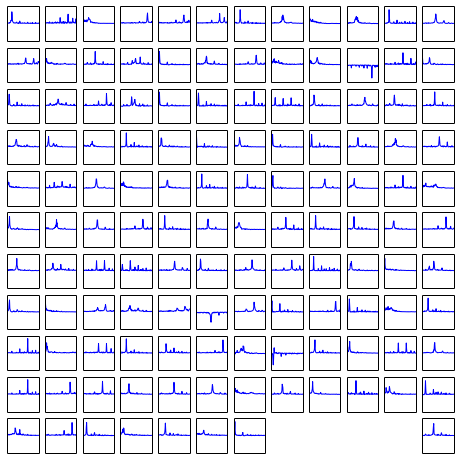
\includegraphics[width=9cm]{img/dictionary}
	\caption[]{A learned dictionary.}
	\label{fig:dictionary}
\end{figure}

\paragraph{Learned dictionary.}
\figref{dictionary} depicts a learned dictionary. Although the atoms are not easily interpretable, single notes seem to appear here and there. \cite{lecun2010PSD} showed that dictionaries trained on individual octaves did discover harmonics, chords and harmonies without any prior about music theory.

\begin{figure}[ht]
	\centering
	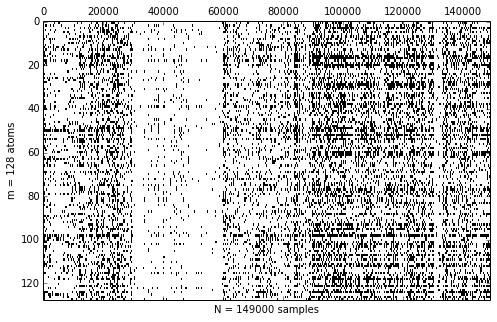
\includegraphics[width=\textwidth]{img/sparse_representations}
	\caption[]{A learned representation, which is indeed sparse.}
	\label{fig:sparse_representations}
\end{figure}

\paragraph{Sparse representations.}
\figref{sparse_representations} shows the representations inferred by \eqnref{model} after convergence. With only 19.8\% of non-zero coefficients, the learned representations are indeed sparse.

\begin{figure}[ht]
	\centering
	\begin{subfigure}[b]{0.9\textwidth}
		\centering
		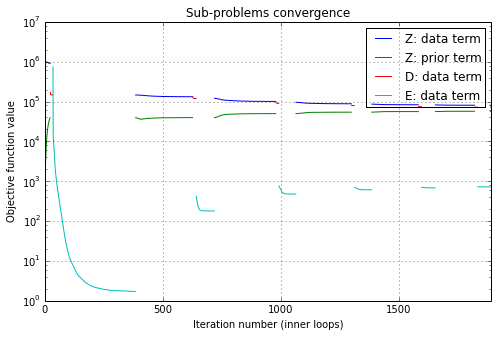
\includegraphics[height=6cm]{img/sub_problems}
		\caption{Sub-problem objectives $f_2(\Z)$, $f_1(\Z)$, $f_2(\D)$ and $f_2(\E)$ evaluated at each inner iteration.}
	\end{subfigure}
	\\
	\begin{subfigure}[b]{0.9\textwidth}
		\centering
		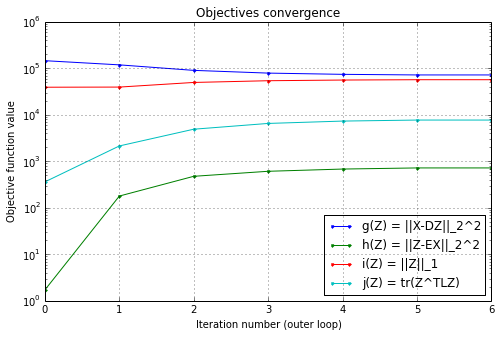
\includegraphics[height=6cm]{img/sub_objectives}
		\caption{Sub-objectives $\fd$, $\fe$, $\fz$ and $\fg$ evaluated at each outer iteration.}
	\end{subfigure}
	\\
	\begin{subfigure}[b]{0.9\textwidth}
		\centering
		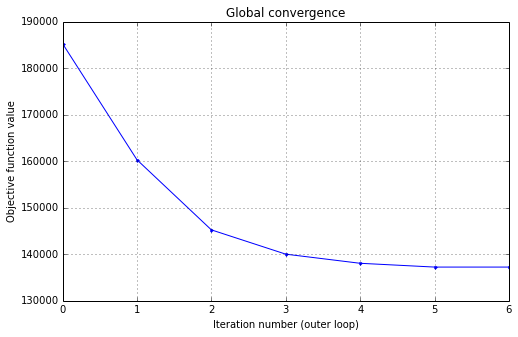
\includegraphics[height=6cm]{img/objective}
		\caption{Global objective $\fd + \fe + \fz + \fg$ evaluated at each outer iteration.}
	\end{subfigure}
	\caption[]{Example of a typical convergence of the algorithm.}
	\label{fig:convergence}
\end{figure}

\paragraph{Convergence.}

While the optimization always end in a different local minimum (\chapref{optimization}), a pretty stable convergence behavior has been observed in all the experiments. \figref{convergence} shows the evolution of the various objectives in a typical convergence of the algorithm.

%The encoder fidelity sub-objective is 2 orders of magnitude lower than the other sub-objectives, which suggests that the addition of the encoder does not alter the features extracted via the complete scheme defined by \eqnref{model}.

%\section{Descriptive features vectors}
% Show aggregated features vectors for some genres.
% How is it qualitatively more discriminative than the spectrogram ?

%\section{Hyper-parameters tuning}
% Test matrix for hyper-parameters on smaller problem (i.e. less frames).
% For ld, le, lg, m
% Numerical parameters: Nouter (enough when no more inner), rtol
% Graph parameters: K, Csigma, kernel?, metric
% Classification: C, Nvectors
% Pre-processing: na=1024, ns=96

% Overcompleteness, defined by the hyper-parameter $m$, must be evaluated by considering the number of code units and the effective dimensionality of the input as given by \gls{PCA}.

%\section{Classification accuracy}
% On the whole dataset, not very good in comparison with others.
% Measured via 10-fold cross-validation
% How classification is improved by features learning, introducing the encoder / graph.
% Comparison with other techniques.
% State what the hyper-parameters are.

%\section{Sparse representations}
% The extracted representations are indeed sparse.

%\section{Scarce training set}
% Il faut juste garder à l'esprit que le graphe (et le dictionnaire) est appris sur le dataset complet. Ça peut cependant être utile si on a beaucoup de données à disposition mais que les labels coûtent chers.

\section{Classification performance}
% Final experiement: baseline, graph-less, graph vs noise level
% Robustness to noisy data

\tabref{classification_accuracy} shows the classification accuracy when using \gls{CQT} spectrograms (the baseline), extracted features with $\lambda_g=0$ (sparse auto-encoder) and $\lambda_g=100$ (structured auto-encoder). The other hyper-parameters are set to $\lambda_z=1$, $\lambda_d=10$ and $\lambda_e=0$.

The first conclusion to draw from this experiment is that the representation extracted from the spectrograms by the structured auto-encoder defined in \partref{algorithm} is indeed more discriminative than the spectrograms themselves in a classification task.

The second conclusion we can draw is that the addition of the smooth prior on the data manifold (\secref{manifold_learning}) always lead to an improved accuracy.

Finally, the sparse and structured representations are robust with respect to noisy data. While a sparse auto-encoder ($\lambda_g=0$) performs even worse than the baseline, our structured auto-encoder ($\lambda_g=100$) out-performs the baseline by 7\%.

\begin {table}[H]
\begin{center}
	\begin{tabular}{|l|c|c|c|c|}
		\hline
		Noise level (standard deviation)  & 0.00 & 0.10 & 0.20 \\
		\hline
		Accuracy (baseline) [\%]          & 69.7 & 58.7 & 46.9 \\
		Accuracy ($\lambda_g=0$) [\%]     & 75.9 & 57.1 & 42.6 \\
		Accuracy ($\lambda_g=100$) [\%]   & 78.0 & 65.9 & 51.6 \\
		\hline
	\end{tabular}
	\caption{Classification accuracies on a subset of GTZAN: $N_{genres} = 5$ genres, $N_{clips} = 100$ clips per genre and $N_{frames} = 149$ frames per clip.}
	\label{tab:classification_accuracy}
\end{center}
\end{table}

%The second experiment shows that structured representations are robust to noise.

%M: However in the noiseless environment the addition of the graph is not significant.
%X: oui, mais tu ne dois pas oublier que tu fais du *transductive* learning, c'est a dire tu apprends les features en utilisant training + TEST data. C'est pour cela que tu n'as pas une amelioration significative. Si on faisait du *supervised* learning, c'est a dire on utilise seulement les TRAINING data, alors ce probleme est bcp plus challenging que le transductive probleme, et la je pense que nos resultats avec graph seraient bien meilleures! C'est un commentaire que je te conseille d'ajouter a ton resultat pour le mettre en perspective. Aussi la premiere chose a faire apres le PDM est de faire du *supervised* learning avec graph et le comparer avec no graph, je pense que l'on aura des (bonnes) surprises!

\section{Discussion}
% Is the model appropriate for the problem ?

While our results are far from the state-of-the-art in \gls{MGR} on GTZAN, we demonstrated the usefulness of an important property of the proposed model: the conservation of the structure in the data. When compared to a sparse auto-encoder, it always leads to a better accuracy, especially in a noisy scenario, when the structure is the most helpful.
%hich allows the system to be robust to noisy data.

We showed experimentally that two assumptions of the model (\secref{assumptions}) are indeed true: the learned representations are sparse (\figref{sparse_representations}) and structured.
%we made the point that our model is useful and that we shall continue to research on it.

Higher classification accuracies are probably achievable by fine-tuning the hyper-parameters and introducing further tricks: e.g. by applying a \gls{LCN} to the \gls{CQT} spectrograms or working on individual octaves, two techniques used by \cite{lecun2011PSDaudio}. We may even further improve the performance of our model by creating a better graph, i.e. a graph more adapted to the problem at hand, by tuning the construction hyper-parameters.


%%%%%%%%%%%%%%%%%%%%%%%%%%%%%%%%%%%%%%%%%%%%%%%%%%%%%%%%%%%%%%%%%%%%%%%%%%%%%%%


\chapter*{Conclusion}
\addcontentsline{toc}{chapter}{Conclusion}
% Discussion of our results. Strengths and weaknesses of our method.

In this work we introduced a novel auto-encoder architecture, which characteristic is to learn sparse and structured representation of input data, borrowing ideas from sparse coding and manifold learning. It learns sparse representations that explicitly take into account the local manifold structure of the data.

The model is formulated as a non-convex optimization problem, for which a well-posed iterative scheme was provided.

The experimental results on music genre recognition showed that our model extracted more discriminant features than sparse auto-encoders.

\section*{Future work}
\addcontentsline{toc}{section}{Future work}
% Split future work on the algorithm and on the application ?
% Only about algorithm ?

\paragraph{Direct encoder.}
% Verify the hypothesis
Our model's third assumption about the existence of a direct encoder (\secref{assumptions}) has to be verified experimentally. It remains to be shown that the features extracted with the approximate scheme \eqnref{z_direct} are equivalent to those extracted with the exact scheme \eqnref{z_exact}. Previous work in the direction however suggests that this assumption is reasonable and that such an encoder should exist.

%\paragraph{TV norm.}
% TV norm on the graph instead of Dirichlet energy

%\paragraph{Distributed implementation.}
% Details ?
% Train chunks of D / Z via independant threads.
% Directly in the PyUNLocBoX ?
% Usefull only if we are not memory bandwidth limited.
% Why ATLAS does not do it by default ? OpenBLAS does it.
% Move to GPU.

%\paragraph{Multiple layers.}
%In the spirit of stacked auto-encoders
% Multiple layers of auto-encoders
% In spite of deep learning methods
% Reference to DBN: stacks of RBM, Stacked auto-encoders.

%\subsection{Deep learning}
% Rebranded as deep learning, achieve now astonishing results in a variety of fields (computer vision, NLP, machine translation, knowledge representation, automatic control)
% Deep learning: hierarchical feature learning --> we are not really using that (yet)
% Deep architectures can approximate any function (RNN any program, i.e. Turing complete)
% First fall of NN (success of kernel methods / SVM) (first AI winter ?) because perceptron was proved to not be sufficient, multi-layer was too hard (computation and training)
% Computationally expensive to train
% Needed to invent backpropagation to train multiple layers
% Hard to train: problem of vanishing gradient
% Objective function is highly non-convex.
% popularized by CNN.

%\paragraph{End-to-end learning.}
% For the application, not the algorithm.
% Learn features right from raw audio. If spectrograms are good features, we should retrieve them.

%\paragraph{Domain knowledge.}
% For the application, not the algorithm.
% Incorporate some domain knowledge about the dictionary via priors. Then it's not supervised anymore.
% Priors on the dictionary who are not necessarily domain specific, i.e. are general enough to apply to other kind of data.

\addcontentsline{toc}{chapter}{References}
\printbibliography

%\chapter*{Annexes}
%\addcontentsline{toc}{chapter}{Annexes}

%\section*{Conference paper}
%\addcontentsline{toc}{section}{Conference paper}
% Draft of ISMIR / ICASSP paper

%\section*{Code}
%\addcontentsline{toc}{section}{Code}
% IPython notebooks exported as LaTex.
% Available on GitHub.

\end{document}